\section{Оборудование}

\begin{figure}[ht!]
    \center{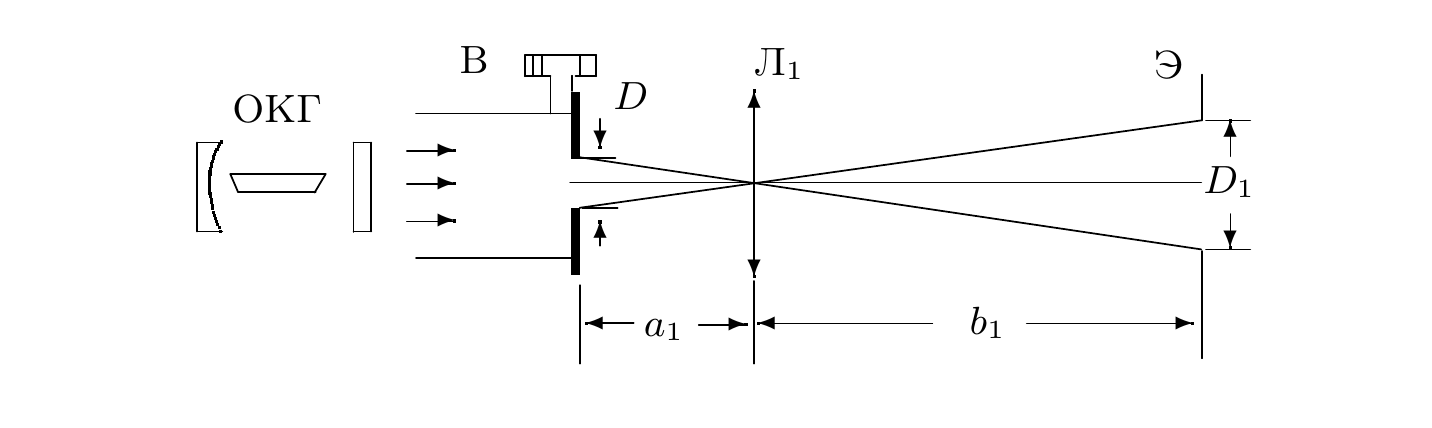
\includegraphics[width=0.8\linewidth]{../img/eq.png}}
\end{figure}
Схема установки представлена на рисунке. Щель переменной ширины $D$,  снабжённая микрометрическим винтом В, освещается параллельным пучком света, излучаемым лазером (радиус кривизны фронта волны велик по сравнению с фокуснымирасстояниями используемых в схеме линз).

Увеличенное изображение щели с помощью линзы $\text{Л}_{1}$ проецируется на экран Э. Величина изображения $D_{1}$ зависит от расстояний от линзы до предмета~--- $a_{1}$ и до изображения~--- $b_{1}$, т.е. от увеличения Г системы
\[
    \Gamma = \frac{D_{1}}{D} = \frac{b_{1}}{a_{1}}
\]

Изображение спектра щели образуется в задней фокальной плоскости Ф линзы $\text{Л}_{1}$. Размещая в плоскости Ф двумерные решётки-сетки, можно влиять на первичное изображение и получать мультиплицированное изображение щели.

Убрав линзу, можно наблюдать на экране спектр щели, а если заменить щель решёткой — спектр решётки. Крупные решётки дают на экране очень мелкую картину спектра, которую трудно промерить. В этом случае используют две линзы: первая (длиннофокусная) формирует первичное изображение~--- спектр, вторая (короткофокусная)~--- проецирует на экран увеличенное изображение спектра.
